\section{Results}\label{sec:Results}

\subsection{Classification}
For logistic regression, we see from table \ref{tab:logreg_allresults} that the way of preprocessing the data which gave the best results was to one hot encode all categorical features and balance the training data such that it contained a $1$:$1$ ratio of the number of defaults and non-defaults, where we have deemed the number of true positive and negative classifications as the most important error metric. The results that follow for logistic regression are based on this preprocessing format of the data. We have done a grid search of the optimal values of the learning rate and number of epochs in the SGD, shown in figure \ref{fig:heatmap_logreg}. The parameters have been evaluated based on the over all accuracy score produced by the model with the respective configuration, which we found to be $0.82$ with a learning rate $ \eta = 10^{-3}$ and $500$ SGD epochs. Table \ref{tab:confusion_logreg} shows the confusion matrix of the models predictions on the test data with this configuration, where it predicted true positives with an accuracy of $0.35$ and true negatives with $0.96$ accuracy. 

\begin{table}[!h]
\label{tab:logreg_allresults}
\caption{Results from classification of the credit card data with logistic regression, in terms of accuracy, area ratio and true positive/negative classifications. Description of the preprocessing methods:\newline
1) One hot encoding of gender, education and marital status.\newline
2) One hot encoding of gender, education, marital status and payment history.\newline
3) Balanced training set with $1$:$1$ ratio of defaults and non-defaults, and one hot encoding of gender, education and marital status.\newline
4) Balanced training set and one hot encoding of gender, education, marital status and payment history.}
\begin{tabular}{|c|c|c|c|c|c|c|}
\hline
Preprocessing method & \multicolumn{2}{c|}{Accuracy} & \multicolumn{2}{c|}{Area ratio} & True positive & True negative \\ \hline
                     & Train          & Test         & Train           & Test          & \multicolumn{2}{c|}{Test}     \\ \hline
1                    & 0.80           & 0.81         & 0.45            & 0.42          & 0.24          & 0.97          \\ \hline
2                    & 0.82           & 0.82         & 0.54            & 0.51          & 0.34          & 0.96          \\ \hline
3                    & 0.81           & 0.80         & 0.46            & 0.44          & 0.26          & 0.97          \\ \hline
4                    & 0.82           & 0.82         & 0.53            & 0.51          & 0.35          & 0.96          \\ \hline
\end{tabular}
\end{table}

%======confusion matrix
\begin{table}[!h]
\caption{Confusion matrix for the predictions of our optimal classifiers on the credit card test data. Label 1 represents default payment, and 0 non-default.}
\label{tab:confusion_logreg}
\begin{tabular}{ccccccccc}
\multicolumn{4}{c}{Logistic regression}                                                                                        &                       & \multicolumn{4}{c}{Neural network}                                                                                            \\ \cline{1-4} \cline{6-9} 
\multicolumn{1}{|c}{}                         & \multicolumn{1}{c|}{}  & \multicolumn{2}{c|}{Prediction}                       & \multicolumn{1}{c|}{} &                                              & \multicolumn{1}{c|}{}  & \multicolumn{2}{c|}{Prediction}                       \\ \cline{3-4} \cline{8-9} 
\multicolumn{1}{|c}{}                         & \multicolumn{1}{c|}{}  & \multicolumn{1}{c|}{0}    & \multicolumn{1}{c|}{1}    & \multicolumn{1}{c|}{} &                                              & \multicolumn{1}{c|}{}  & \multicolumn{1}{c|}{0}    & \multicolumn{1}{c|}{1}    \\ \cline{1-4} \cline{6-9} 
\multicolumn{1}{|c|}{\multirow{2}{*}{Actual}} & \multicolumn{1}{c|}{0} & \multicolumn{1}{c|}{0.96} & \multicolumn{1}{c|}{0.04} & \multicolumn{1}{c|}{} & \multicolumn{1}{c|}{\multirow{2}{*}{Actual}} & \multicolumn{1}{c|}{0} & \multicolumn{1}{c|}{0.92} & \multicolumn{1}{c|}{0.08} \\ \cline{2-4} \cline{7-9} 
\multicolumn{1}{|c|}{}                        & \multicolumn{1}{c|}{1} & \multicolumn{1}{c|}{0.65} & \multicolumn{1}{c|}{0.35} & \multicolumn{1}{c|}{} & \multicolumn{1}{c|}{}                        & \multicolumn{1}{c|}{1} & \multicolumn{1}{c|}{0.36} & \multicolumn{1}{c|}{0.64} \\ \cline{1-4} \cline{6-9} 
\end{tabular}
\end{table}
%=====

\begin{figure}[!h]
    \centering
    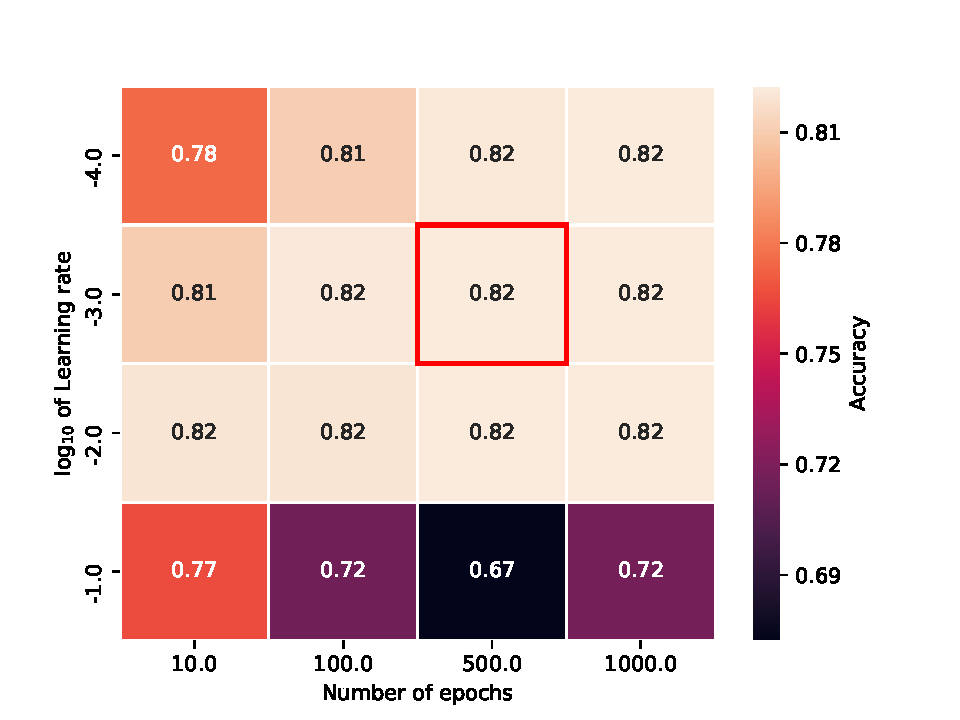
\includegraphics[scale=0.6]{Figures/Classification/020_logistic_heatmap_CC_bal_all1h_on_val.pdf}
    \caption{Heat map of the grid search for best learning rate and no. of epochs with logistic regression on the credit card data. Each of the data points have been found using k-fold cross validation with $k=5$ for a better estimation of the accuracy.}
    \label{fig:heatmap_logreg}
\end{figure}


For our neural network classifier, we found an optimal learning rate for the model to be $\eta = 10^{-1}$, shown in figure \ref{fig:eta_epoch_analysis_nn}. The figure also shows that the best way of data preprocessing is to one hot encode all categorical features and balance the training data in terms of number of defaults/non-defaults. Based on these parameters, we have done a grid seach of the optimal number of hidden layers and nodes per layer in the neural network, shown in figure \ref{fig:heatmap_nn_classification}, where we see that the  optimal configuration is three hidden layers with $80$ nodes each. Table \ref{tab:confusion_logreg} shows the confusion matrix of our final model, trained with the parameters found above and $10.000$ SGD epochs, giving a true positive rate of $0.64$, true negative rate of $0.92$ and an accuracy score of $0.86$ on the test data. 

In table \ref{tab:results_classification} we have listed the results from our best classifiers and for comparison those of I-C Yeh, C-h Lien\cite{YehLien}[p.5]. In the case of logistic regression, we see that out results are very similar in terms of accuracy ($0.81$ vs $0.82$ on the test data), though we achieve a higher area ratio with our model ($0.51$ vs $0.44$ on the test data). For neural networks, our optimal model has an accuracy score of $0.86$ on the test data, while Yeh and Lien's is $0.83$. We also achieve a higher area ratio with our model ($0.65$ vs $0.54$ on the test data). The gain charts of our classifiers are shown in figures \ref{fig:gain_logreg_nn}.

\begin{figure}[!h]
    \centering
    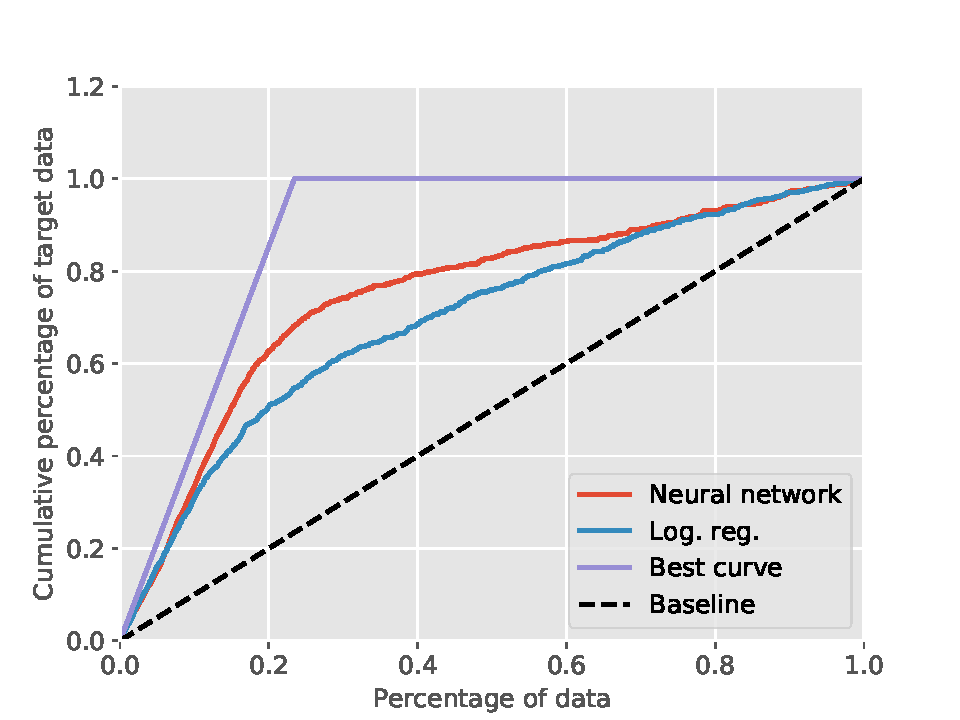
\includegraphics[scale=0.6]{Figures/Classification/gain_chart.pdf}
    \caption{Gain curves of our classifiers on the credit card test data. The blue curve shows the results for logistic regression (area ratio $0.51$), the red curve shows the results for neural network (area ratio $0.65$).}
    \label{fig:gain_logreg_nn}
\end{figure}





%======================================================
% Neural network result figures
\begin{figure}[!h]
    \centering
    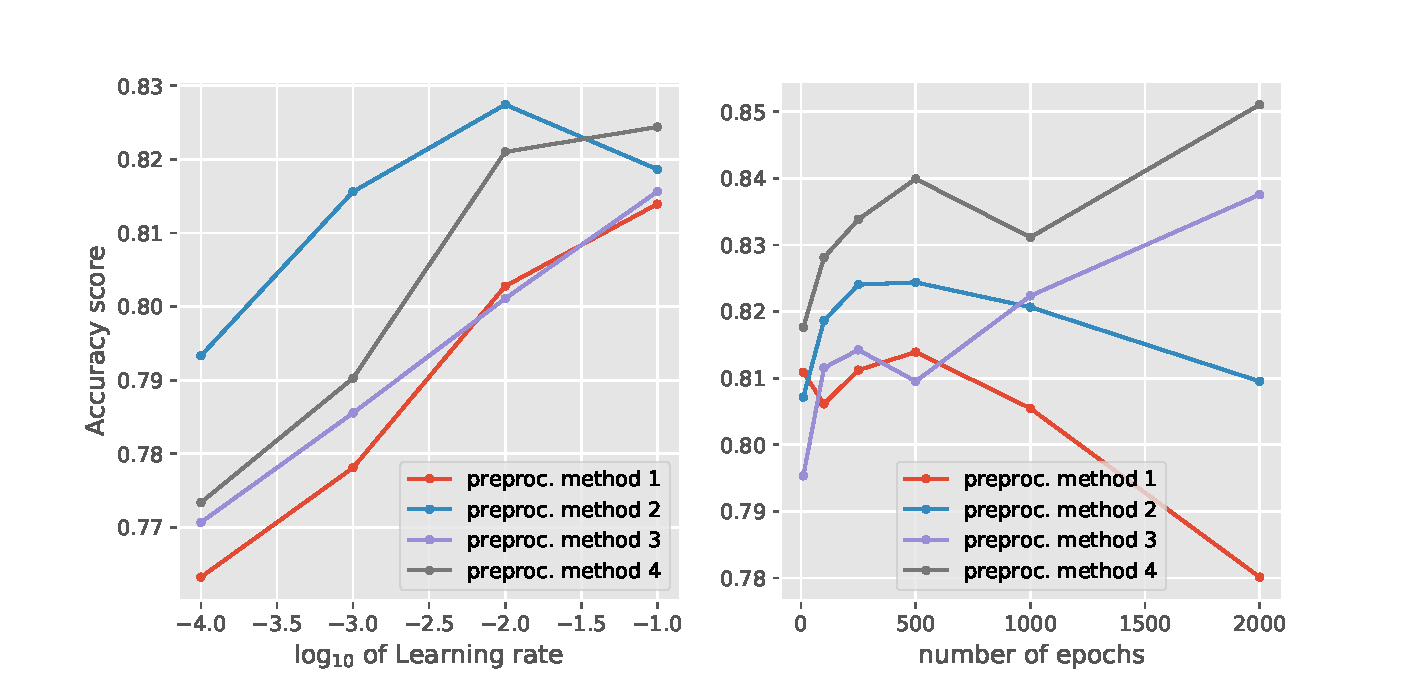
\includegraphics[scale=0.6]{Figures/Classification/class-eta-accuracy_full_analysis_analysis2.pdf}
    \caption{Accuracy score when testing a neural network with varying learning parameter and number of epochs, using 3 layers with 100 nodes in each. The best performing learning rate (in terms of accuracy score) were selected from the left plot, which were $\eta = 10^{-1}$, and this value was used when producing the plot to the right. In the initial analysis in the left plot we used 100 epochs when training the network. The preprocessing methods are as defined in the caption of table \ref{tab:classification_results_bad}.}
    \label{fig:eta_epoch_analysis_nn}
\end{figure}
\begin{figure}[!h]
    \centering
    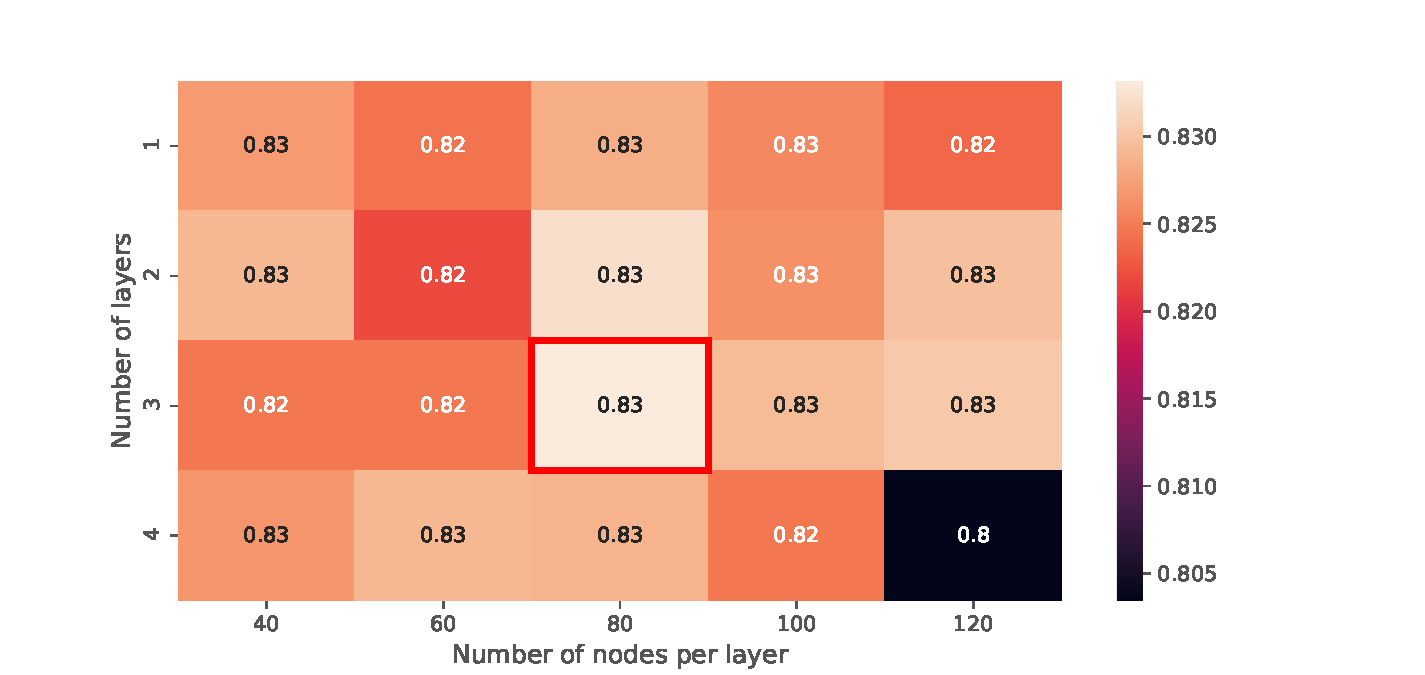
\includegraphics[scale=0.6]{Figures/Classification/class_heatmap_analysis2_hl-100-100-100_maxepochsoptimal10000.pdf}
    \caption{Heat map of grid search for configuration of number of layers and nodes per layer when using a neural network. The highest accuracy score obtained is marked with red rectangle. In this grid search we have used $100$ epochs in the SDG and a learning rate $\eta = 10^{-1}$.}
    \label{fig:heatmap_nn_classification}
\end{figure}

%======================================================


\begin{table}[!h]
\label{tab:results_classification}
\caption{Classification results from logistic regression and classification.}
\begin{tabular}{cccccccccc}
                                          & \multicolumn{4}{c}{Our models}                                                                                            &                       & \multicolumn{4}{c}{I-C Yeh, C-h Lien}                                                                                 \\ \cline{1-5} \cline{7-10} 
\multicolumn{1}{|c|}{Method}              & \multicolumn{2}{c|}{Accuracy}                               & \multicolumn{2}{c|}{Area ratio}                             & \multicolumn{1}{c|}{} & \multicolumn{2}{c|}{Accuracy}                             & \multicolumn{2}{c|}{Area ratio}                           \\ \cline{1-5} \cline{7-10} 
\multicolumn{1}{|c|}{}                    & \multicolumn{1}{c|}{Training} & \multicolumn{1}{c|}{Test}   & \multicolumn{1}{c|}{Training} & \multicolumn{1}{c|}{Test}   & \multicolumn{1}{c|}{} & \multicolumn{1}{c|}{Training} & \multicolumn{1}{c|}{Test} & \multicolumn{1}{c|}{Training} & \multicolumn{1}{c|}{Test} \\ \cline{1-5} \cline{7-10} 
\multicolumn{1}{|c|}{Logistic regression} & \multicolumn{1}{c|}{0.82}     & \multicolumn{1}{c|}{0.81}   & \multicolumn{1}{c|}{0.53}     & \multicolumn{1}{c|}{0.51}   & \multicolumn{1}{c|}{} & \multicolumn{1}{c|}{0.80}     & \multicolumn{1}{c|}{0.82} & \multicolumn{1}{c|}{0.41}     & \multicolumn{1}{c|}{0.44} \\ \cline{1-5} \cline{7-10} 
\multicolumn{1}{|c|}{Neural Network}      & \multicolumn{1}{c|}{0.98}   & \multicolumn{1}{c|}{0.86} & \multicolumn{1}{c|}{0.99}   & \multicolumn{1}{c|}{0.65} & \multicolumn{1}{c|}{} & \multicolumn{1}{c|}{0.81}     & \multicolumn{1}{c|}{0.83} & \multicolumn{1}{c|}{0.55}     & \multicolumn{1}{c|}{0.54} \\ \cline{1-5} \cline{7-10} 
\end{tabular}
\end{table}













\subsection{Regression}
For our regression case, where we used a data set generated by the Franke function, the initial analysis of the learning parameter is shown in the left plot in figure \ref{fig:eta_epoch_analysis_nn_regression}, which were found to be $10^{-2}$ when using the ReLU as activation function. The sigmoid function was also tested for the same values of the learning rate, excluding $10^{-1}$ because the gradient diverged, and we were not able to get a result. We then performed an analysis of how the mean squared error behaved as a function of number of epochs, as shown in the right plot in figure \ref{fig:eta_epoch_analysis_nn_regression}. Figure \ref{fig:heatmap_nn_regression} shows a grid search of the optimal configuration of number of layers and number of nodes in each layer. The best performing configuration from this analysis is then used in figure \ref{fig:franke20}, where we see a plot of the generated data as a 3D surface, with the neural network prediction as a wiregrid on top. In this case we used $2000$ epochs to produce the results, because we observed slightly better results when increasing the number of epochs. Table \ref{tab:regression} shows the MSE and $R^2$ score for our neural network, compared with the regression methods which we used in our previous project\cite{project1}. In all of the figures and tables mentioned in this section, the MSE and $R^2$ score is measured on the test set of the data, which consists of 20\% of the full data set.

In figure \ref{fig:regression_gridsize} we see a plot of how the performance metrics MSE and $R^2$ behaves as a function of the grid size of our Franke data set which is sent through our neural network. The figure caption contains the parameters used when creating the models.

\begin{figure}[!h]
    \centering
    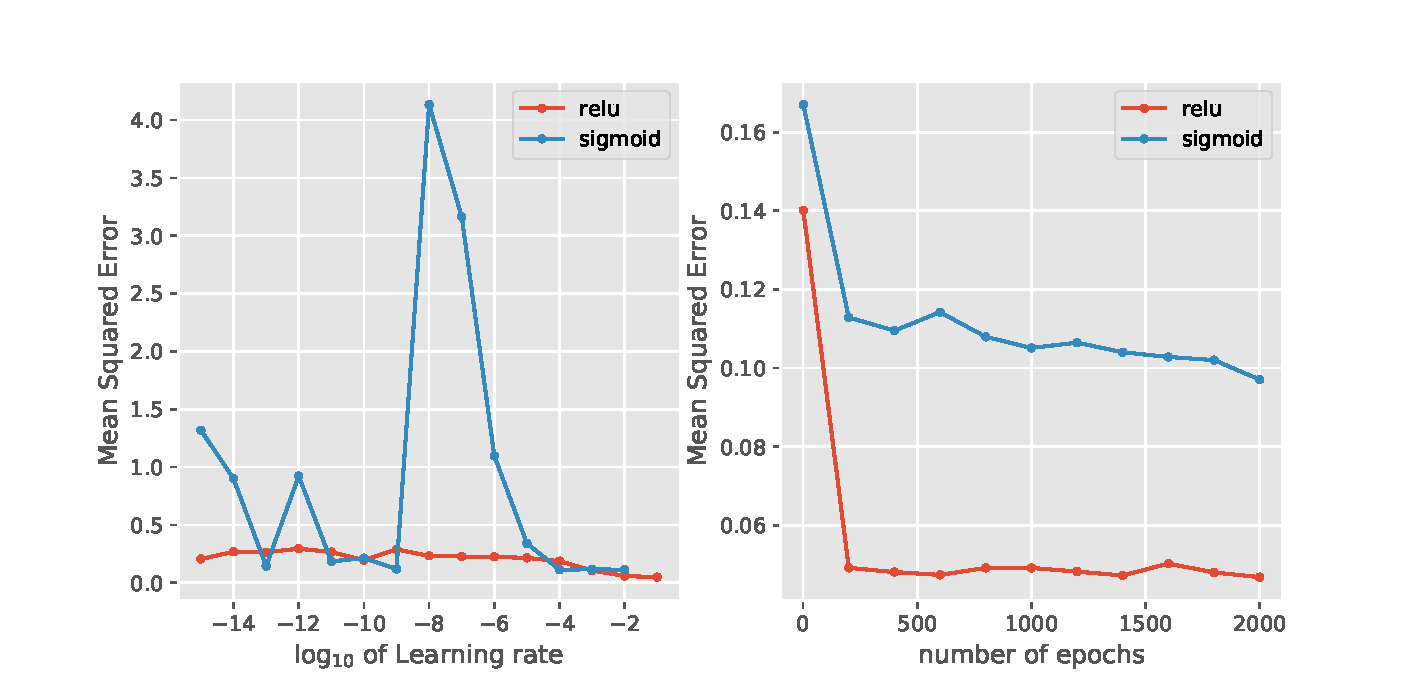
\includegraphics[scale=0.6]{Figures/Regression/eta-mse_l100-100_epochs500.pdf}
    \caption{MSE of the test set when testing a neural network with varying learning parameter and number of epochs on the Franke data set, using both ReLU and sigmoid as activation function. The best performing learning rate was found to be $10^{-1}$ in the left plot, and this learning rate was used when analyzing number of epochs in the right plot. In all of these cases we used two layers with 100 nodes in each.}
    \label{fig:eta_epoch_analysis_nn_regression}
\end{figure}
\begin{figure}
    \centering
    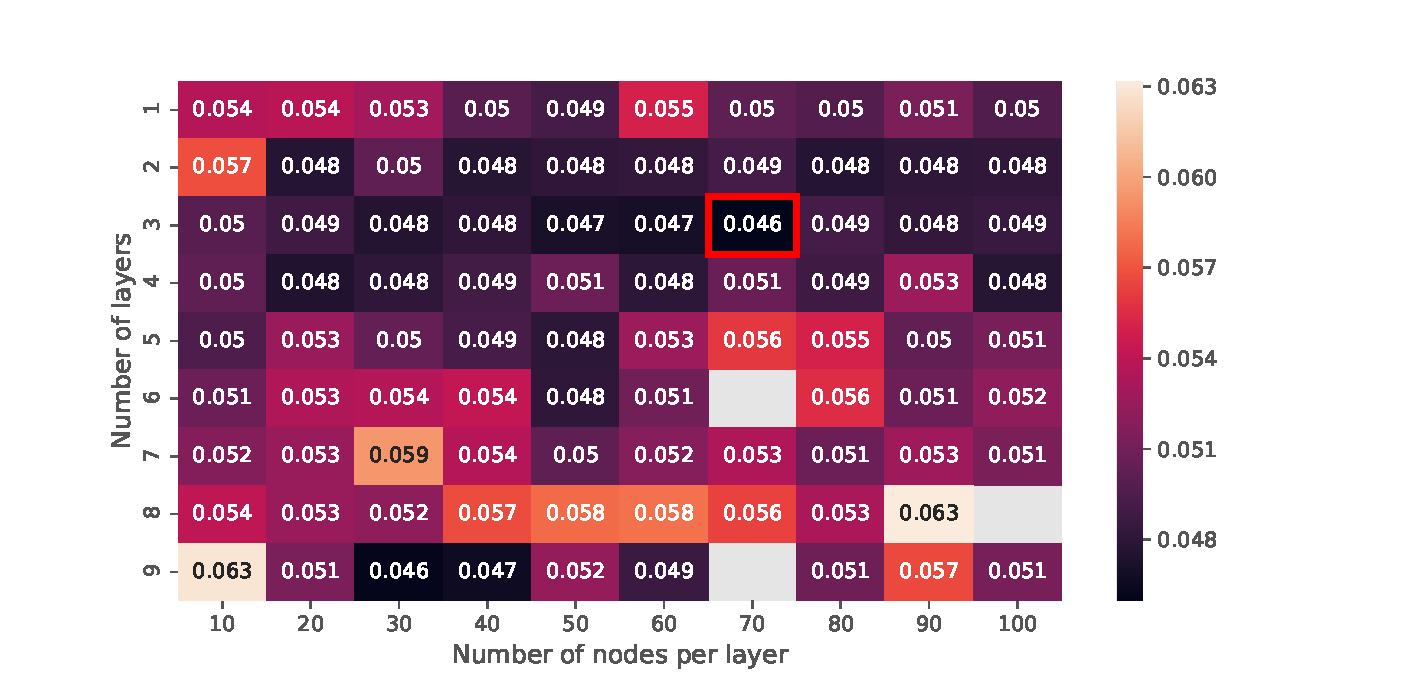
\includegraphics[scale=0.6]{Figures/Regression/heatmap_epochs500_layers10.pdf}
    \caption{Heat map of grid search for configuration of number of layers and nodes per layer when using a neural network with learning rate of $10^{-1}$ and 500 SGD epochs. The lowest MSE obtained on the test set is marked with red rectangle. The blank grey boxes indicate cases where the gradient exploded during the training of the network, and no result were obtained.}
    \label{fig:heatmap_nn_regression}
\end{figure}
\begin{figure}
    \centering
    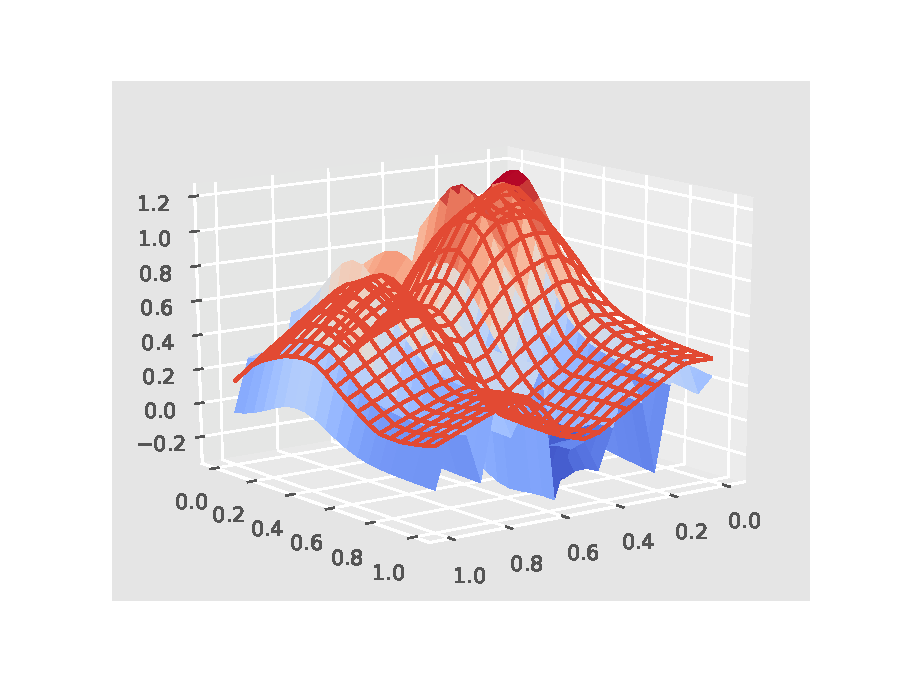
\includegraphics[scale=0.7]{Figures/Regression/nn_franke_optimal_n20.pdf}
    \caption{The Franke data (solid surface), with gridsize $20 \times 20$ and a noise of $\epsilon=0.2$, plotted together with the prediction from the neural network (wiregrid), using 3 hidden layers with 70 nodes each on a run of $10000$ epochs. }
    \label{fig:franke20}
\end{figure}

\begin{table}[]
    \centering
    \caption{Comparison of MSE and $R^2$ score (measured on the test set) between the three different regression methods used in our previous project\cite{project1} and the neural network, when used to model data generated from the Franke function.}
    \begin{tabular}{|c|c|c|}
        \hline
        Method          & MSE       & $R^2$ \\
        \hline
        OLS             &  0.0136   & 0.819  \\ 
        \hline
        Ridge           & 0.0139    & 0.877  \\ 
        \hline
        Lasso           & 0.0183    & 0.728  \\
        \hline
        Neural network  &    0.0415   & 0.631 \\
        \hline
    \end{tabular}
    \label{tab:regression}
\end{table}


\begin{figure}
    \centering
    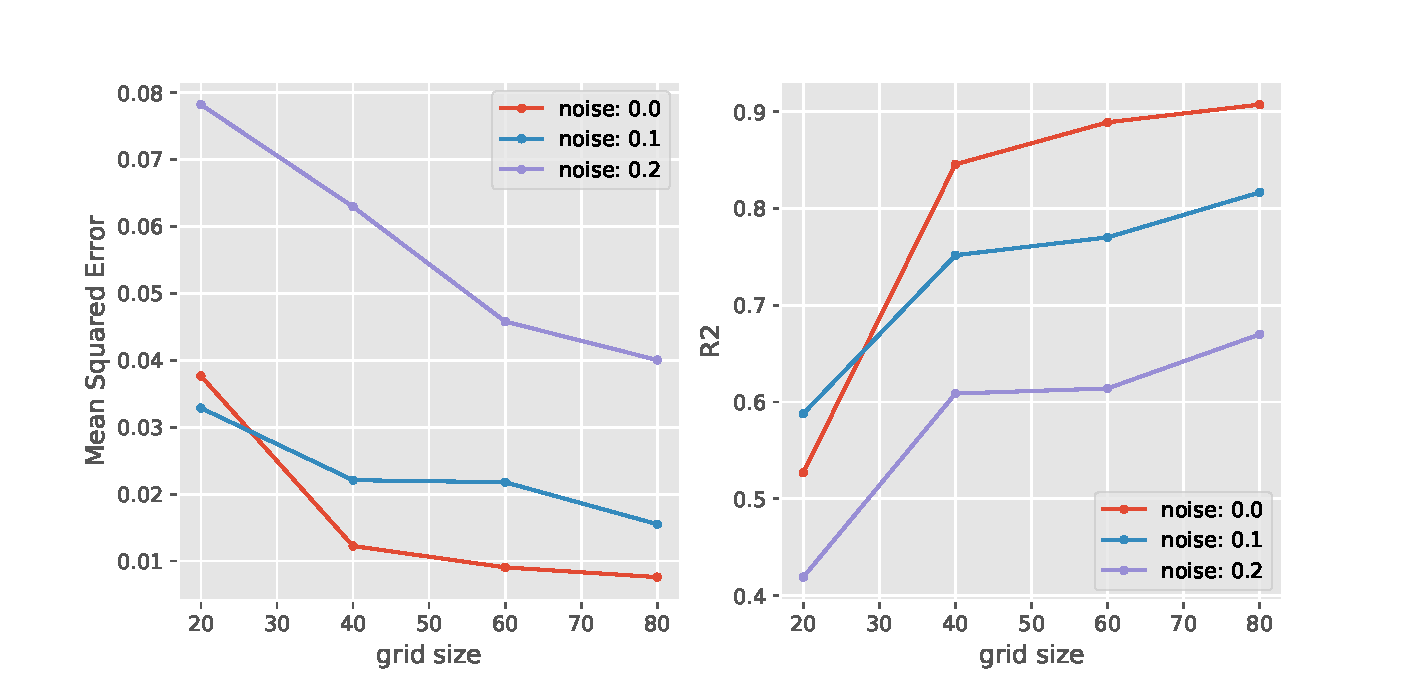
\includegraphics[scale=0.65]{Figures/Regression/grid-mse-analysis7.pdf}
    \caption{MSE and $R^2$ score (measured on the test set) as a function of the grid size of the Franke function, for three different values of noise introduced to the data set, when a neural network with 3 hidden layers of 70 nodes each, and a learning parameter of $10^{-1}$, is applied to the data set, over 200 epochs.}
    \label{fig:regression_gridsize}
\end{figure}